\documentclass{article}
\usepackage[english]{babel}

\usepackage[a4paper,top=2cm,bottom=2cm,left=2cm,right=2cm,marginparwidth=1.75cm]{geometry}
\usepackage{graphicx}
\title{SSL/TLS Presentation}
\author{Federico Luisetto}
\begin{document}
\maketitle

%SSL/TLS
\section{What's SSL/TLS}
Transport Layer Security (TLS), the successor of the now-deprecated Secure Sockets Layer (SSL), is a cryptographic 
protocol designed to provide communications security over a computer network. Several versions of the protocol are widely 
used in applications such as email, instant messaging, and voice over IP, but its use as the Security layer in HTTPS remains the most publicly visible.
\\The TLS protocol aims primarily to provide privacy and data integrity between two or more communicating computer applications.
\\The TLS protocol comprises two layers: the SSL record protocol and the Upper Layer Carrying.\\\\

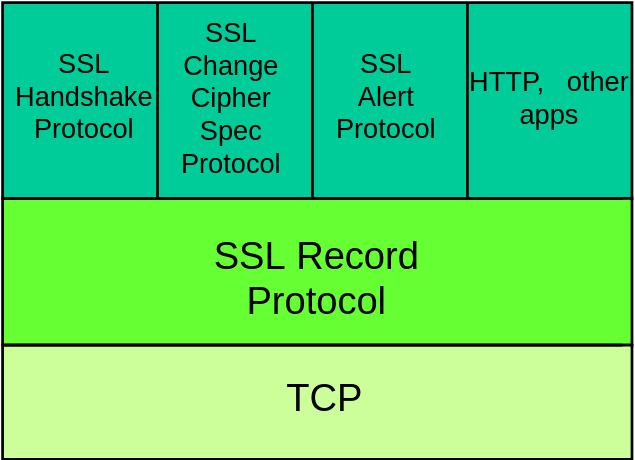
\includegraphics[width=8cm]{SSL_TLS.png}

%SSL record protocol
\section{SSL Record Protocol}
SSL Record Protocol provides secure, reliable channel for upper layer.
It carries application data and SSL 'management' data.\\
It provides:
\begin{itemize}
    \item Data origin authentication and integrity
    \begin{itemize}
        \item MAC using algorithm similar to HMAC
        \item Based on MD5 or SHA-1 hash algorithms
        \item MAC protects 64 bit sequence number for anti-replay
    \end{itemize}
    \item Confidentiality
    \begin{itemize}
        \item Bulk encryption using symmetric algorithm
        \begin{itemize}
            \item DEA, RC2-40, DES-40 (exportable), DES, 3DES
            \item RC4-40 and RC4-128
        \end{itemize}
    \end{itemize}
\end{itemize}
Process:
\begin{enumerate}
    \item Data from application/upper layer SSL protocol partitioned into fragments (max size 214 bytes)
    \item MAC first then pad (if needed)
    \begin{itemize}
        \item MAC (Message Authentication Code) is a short piece of information used to authenticate a message
    \end{itemize}
    \item Encrypt
    \item Append header (Content type, version, length of fragment)
    \item Submit to TCP
\end{enumerate}
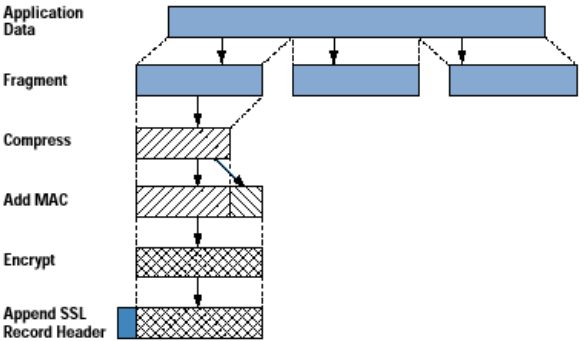
\includegraphics[width=8cm]{SSL_Record_Protocol.png}

%Upper Layer Carrying
\section{Upper Layer Carrying}

\subsection{SSL Handshake Protocol}
\begin{enumerate}
    \item Client \textit{hello} packet
    \begin{itemize}
        \item Client announces its capabilities (cipher list, compression methods, highest SSL/TLS version).
        \\es: TLS\_RSA\_WITH\_3DES\_EDE\_CBC\_SHA
        \item Sends ClientNonce (28 random bytes plus 4 bytes of time)
        \item Session ID
    \end{itemize}
    \item Server \textit{hello} packet
    \begin{itemize}
        \item Selects single ciphersuite from list offered by client
        \\es: TLS\_RSA\_WITH\_3DES\_EDE\_CBC\_SHA
        \item Sends ServerNonce and SessionID
    \end{itemize}
    \item Server sends its public certificate to client
    \item Server \textit{hello done} packet
    \item Client send \texttt{pre\_master\_secret} key to server
    \begin{itemize}
        \item This key is encrypted using server's public key
    \end{itemize}
    \item Generation of symmetric key
    \begin{itemize}
        \item Client and server generate the Master Secret and session keys based on the Pre-Master Secret
    \end{itemize}
    \item Update of ChipherSpec for this session
    \begin{itemize}
        \item Client and server change the ChipherSpec to symmetric encryption using the session key
    \end{itemize}
\end{enumerate}
\subsection{SSL Change Cipher Spec}
The Change Cipher Spec Protocol is used to change the encryption being used by the client and server. 
It is normally used as part of the handshake process to switch to symmetric key encryption. 
The CCS protocol is a single message that tells the peer that the sender wants to change to a new set of keys, 
which are then created from information exchanged by the handshake protocol.
\subsection{SSL Alert Protocol}
The alert protocol is used to alert status changes to the peer. The primary use of this protocol is to report the cause of failure. 
Status changes include such things as error condition like invalid message received or message cannot be decrypted, as well as things 
like the connection has closed. One thing that TLS has over SSL is that TLS has more alert messages than SSL does.
\end{document}

